\chapter{Resultaten}
%\label{resultaten-origineel}

In dit hoofdstuk bespreken we de testen die een antwoord geven op de onderzoeksvraag en hypotheses. In sectie \ref{opstelling} worden enkele praktische zaken besproken. Daarna worden de drie besproken technieken uit hoofdstukken \ref{blcf} en \ref{nlcf} onderling vergeleken.

\section{Opstelling}
\label{opstelling}
Deze masterproef maakte gebruik van de offici\"ele GTFS dataset van de Belgische spoorwegenmaatschappij NMBS. 

Zowel de cli\"ent als de server werden getest op dezelfde machine: een Macbook Pro 2015 editie met 8 GB RAM en Intel Core i5 2,7 Ghz processor. De cli\"ent is een webapplicatie waarin queries werden uitgevoerd. Als browser werd Firefox gebruikt.

%\begin{itemize}
%\item NMBS: de Belgische spoorwegen
%\item NS: de Nederlandse spoorwegen
%\item De Lijn: busnetwerk in Vlaanderen
%\end{itemize}

%Eerst zullen we testen hoe basic LDF scoort bij de NMBS afzonderlijk. Daarna testen we de \textit{merger} (zie \ref{merger}) uit door NMBS en NS samen te voegen. 
%Als slot kun we onze benchmarks op de dataset van De Lijn uitvoeren. Deze laatste bestaat uit een groter netwerk van stops dan NMBS en NS samen en bevat een grotere hoeveelheid connecties per dag.

%\section{Interoperabiliteit}
%Om meerdere operatoren te kunnen gebruiken is er een mapping van stops die dicht bij elkaar liggen nodig. Een use case in de praktijk moet rekening houden met bepaalde overstaptijden (Engels: \textit{transfer time}). Wegens de complexiteit van deze stops wordt dit achterwege gelaten en wordt er een minimale overstaptijd van 0 minuten ingesteld. Stops die op een afstand van minder dan 200 meter liggen, krijgen een nieuwe stop identifier, zogenaamde connectie stop identifier. Een afstand van 200 meter is nodig, omdat bushaltes van een groot station zoals Antwerpen-Centraal ver uit elkaar liggen.
%Dit mappen naar een connectie stop identifier gebeurt voor het genereren van connecties.
%
%\section{Opstelling}
%Voor elke dataset is een Docker-container opgezet. Dit zijn virtuele machines waarin de software kan lopen. De cli\"ent is een webapplicatie die in het hoofdbesturingssysteem draait. De testen zijn uitgevoerd op een Macbook Pro 2015 editie met 8 GB RAM en Intel Core i5 2,7 Ghz.

% todo tekening docker

\subsection{Lokale server versus productieserver}

Doordat de testen werden uitgevoerd in een lokale omgeving zullen we testen of er een merkbaar verschil in snelheid is met een server in productie\footnote{Linked Connections server te vinden op: http://belgianrail.linkedconnections.org/connections/}. 
Er werden een honderdtal queries op de dataset van de NMBS uitgevoerd. Beide servers hebben als  tijdsinterval tien minuten.

\begin{table}[htbp]
\centering
\begin{tabular}{ | c || c | c | c | c | c | }
  \hline
  Type & Aantal queries & Querytijd (s) & Requests & Querytijd/request (s) & Connecties \\ \hline
  lokaal & 30 & 103.196 & 583 & 0.17 & 10368 \\
  productie & 30 & 68.5509 & 550 & 0.12 & 9915 \\
\hline  
\end{tabular}
\caption{Vergelijking tussen een lokale server een productieserver.}
\label{table:vglservers}
\end{table}

Figuur \ref{table:vglservers} toont aan dat er een verschil in snelheid is tussen een lokale en een productieserver. Dezelfde queries werden berekend met een verschillende vertrekdatum. Dit is de reden waarom het aantal requests en connecties niet gelijk zijn.
Het resultaat toont aan dat lokale server 30\% trager dan een productieserver is. Volgende subsectie toont aan welke fragmentgrootte gemiddeld het snelst is.

%\subsection{Scannen versus requests}
%
%De cli\"ent is verantwoordelijk voor het ophalen van connecties met HTTP requests die vervolgens gescant worden door CSA. Volgende hypothese wordt beantwoord:
%
%\begin{itemize}
%\item \emph{}
%\end{itemize}


\subsection{Fragmentgrootte}
\label{fragmentgrootte}

\textit{Basic Linked Connections Fragment's} (BLCF) hebben een vast tijdsinterval waarin connecties worden teruggeven. Dit komt met een gemiddeld aantal connecties. Tabel \ref{table:grootte-tijd} toont een overzicht van verschillende fragmentgroottes die mogelijk zijn met de hoeveelheid data die er gemiddeld aan verbonden is.

%\begin{table}[htbp]
%\centering
%\begin{tabular}{ | c || c | c | c | c | c | c | c | }
%  \hline
%  & \multicolumn{2}{|c|}{NMBS} & \multicolumn{2}{|c|}{NS} & \multicolumn{2}{|c|}{De Lijn} \\ \hline
%  t (min) &	Grootte (MB) &	Connecties & Grootte & Aantal connecties & Grootte & Connecties \\ \hline
% 1 &	0.012 & 56 & 0.017 & 46 & 0.25 & 975 \\
% 2 &	0.027 & 115 & 0.029 & 104 & 0.49 & 1904  \\
% 5 & 0.069 & 264 & 0.068 & 262 & 1.23 & 4833 \\
%10 &	0.14 & 570 & 0.13 & 522 & 2.47 & 9603 \\
%20 &	0.27 & 1144 & 0.25 & 1019 & 4.21 & 16441 \\
%30 & 0.41	& 1704 & 0.37 & 1539 & 6.23 & 24813 \\
%40 &	0.55	& 2281 & 0.51 & 2045 & 8.33 & 33309 \\
%80 &	1.10	& 4564 & 1.00 & 4126 & 18.71 & 66432 \\
%120 & 1.90 & 7356 & 1.51 & 6267 & 27.29 & 100314 \\
%160 & 2.21 & 9332 & 2.04 & 8075 & 35.82 & 135960 \\
%200 & 2.77 & 11419 & 2.56 & 10512 & 44.37 & 169619 \\	
%\hline  
%\end{tabular}
%\caption{Grootte (MB) en aantal connecties afhankelijk van tijdsinterval van basic LCF.}
%\label{table:grootte-tijd}
%\end{table}

\begin{table}[htbp]
\centering
\begin{tabular}{ | c || c | c | c | c | c | c | c | }
  \hline
  & \multicolumn{2}{|c|}{NMBS} \\ \hline
  t (min) &	Grootte (MB) &	Connecties \\ \hline
 1 &	0.012 & 56  \\
 2 &	0.027 & 115  \\
 5 & 0.069 & 264  \\
10 &	0.14 & 570  \\
20 &	0.27 & 1144 \\
30 & 0.41	& 1704  \\
40 &	0.55	& 2281  \\
80 &	1.10	& 4564  \\
120 & 1.90 & 7356  \\
160 & 2.21 & 9332  \\
200 & 2.77 & 11419  \\	
\hline  
\end{tabular}
\caption{Grootte (MB) en aantal connecties afhankelijk van tijdsinterval van basic LCF.}
\label{table:grootte-tijd}
\end{table}

\begin{figure}[!tbp]
  \centering
  \subfloat[De gemiddelde tijd in seconden om queries uit te voeren in functie van het tijdsinterval van basic LCF.]{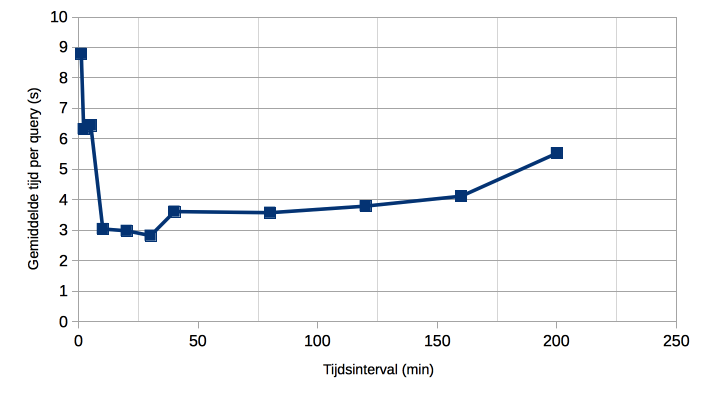
\includegraphics[width=0.5\textwidth]{relatie-tijdsinterval-tijdperquery}\label{fig:relatie-tijdsinterval-tijdperquery}}
  \hfill
  \subfloat[De hoeveelheid opgevraagde data in megabyte in functie van het tijdsinterval van basic LCF.]{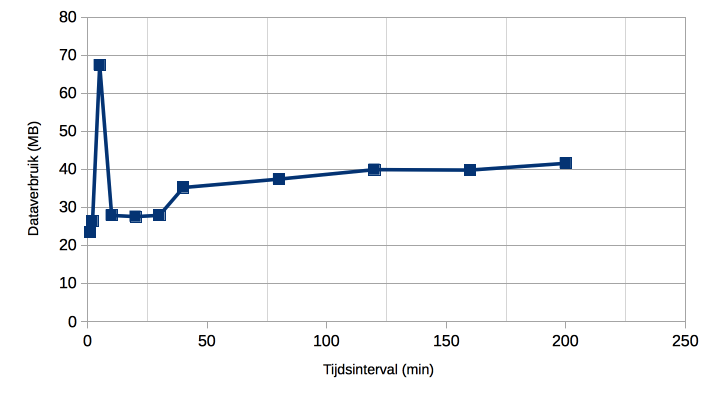
\includegraphics[width=0.5\textwidth]{relatie-tijdsinterval-grootte}\label{fig:relatie-tijdsinterval-grootte}}
  \caption{Snelheid en grootte hangen af van de ingestelde tijdsinterval van basic Linked Connections Fragments.}
  \label{fig:fragmentgrootte}
\end{figure}

Om te bepalen wat de optimale fragmentgrootte is, werden een honderd queries uitgevoerd met telkens een andere fragmentgrootte. De resultaten in \ref{fig:fragmentgrootte} tonen aan dat een tijdsinterval tussen 10 en 30 minuten de gemiddeld beste querysnelheid geeft. Dit komt overeen met een paginagrootte van 500 tot 2000 connecties. Figuur \ref{fig:relatie-tijdsinterval-grootte} toont een lineair verband tussen het aantal gedownloade fragmenten en het ingestelde tijdsinterval. Bij zeer kleine fragmenten kunnen er uitschieters ontstaan.

De grootte van een fragment is afhankelijk van het aantal aanwezige connecties. Zo (zie Tabel \ref{table:grootte-connectie}) is er een gemiddelde vaste grootte per connectie. Deze zal later gebruikt worden als referentie-waarde.

 \begin{table}[htbp]
\centering
\begin{tabular}{ | c | c | c | }
  \hline
   & Kilobyte & Megabyte \\ \hline
 Grootte connectie & 0,26158 & 0,00026158 \\
\hline  
\end{tabular}
\caption{Grootte van een connectie.}
\label{table:grootte-connectie}
\end{table}


Uit \ref{fig:fragmentgrootte} kan ook afgeleid worden dat de snelheid van routeplanning afhankelijk is van de combinatie van het aantal connecties en het aantal requests. Voor korte routes zijn kleinere fragmentgroottes beter. Lange routes zijn veel sneller met minder requests en een groot tijdsinterval. Om niet te groot contrast te hebben tussen korte en lange routes, moet er dus een gulden middenweg genomen worden van rond de 1500 connecties per fragment. Hierbij moet er ook zuinig omgegaan worden met data. Grote overschotten van connecties die niet gescant moeten worden, zijn te vermijden.

Voortaan zullen we als referentie pagina's van ongeveer 1000 connecties nemen. In tabel \ref{overzicht-fragmentgroottes} staat een overzicht van de verschillende paginagroottes voor de drie technieken die getest zijn. Voor NLCF is een verschillende grootte voor de gecachete snelheidstest en niet-gecachte. Het aantal mogelijke overstappen $K$ is gemaximaliseerd zodat elke stop bereikbaar is vanuit een bepaalde vertrekstop. Voor de NMBS is $max K = 5$.

\begin{table}[htbp]
\centering
\begin{tabular}{ | c || c | c | c | c |}
  \hline
  Techniek & BLCF (min) & NLCF cache (min)& NLCF zonder cache & Fragmentgrootte (min) \\ \hline
  Basic LCF & 20 & - & - & - \\
  Speed-up & 20 & 30 & 40 & 120 \\
  Heuristiek & 20 & 100 & 100 & 100 \\
\hline
\end{tabular}
\caption{Tijdsintervallen voor de verschillende technieken.}
\label{table:tijdsintervallen}
\end{table}

De reden waarom het tijdsinterval van NLCF's beperkt blijft tot 100-120 minuten is omdat dit kostelijker is voor de server om te berekenen. Zo moet er een extra databank-request gestuurd worden om de buren op te vragen van een stop. Na 120 minuten zijn de meeste stopplaatsen al bereikbaar waardoor deze soort fragmenten niet meer opwegen in snelheid.

\section{Hypotheses}
Volgende twee hypotheses worden aangekaard:

\begin{itemize}
\item \emph{Hoe meer connecties, hoe meer bandbreedte. Bijgevolg meer tijd.}
\end{itemize}

\begin{figure}[!tbp]
  \centering
  \subfloat[HTTP requests in functie van aantal connecties.]{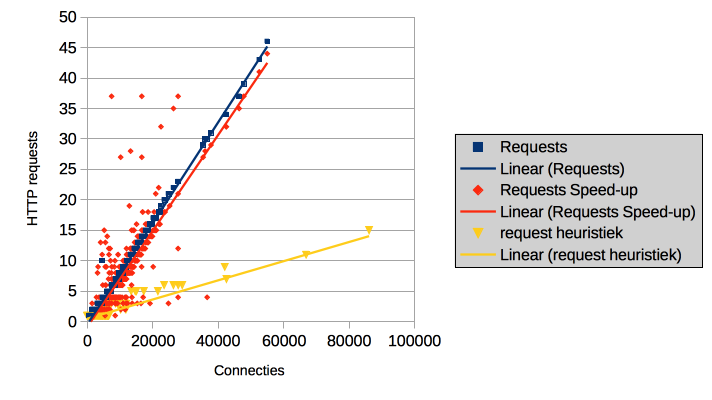
\includegraphics[width=0.5\textwidth]{aantalrequestsvolgensconnecties}\label{fig:aantalrequestsvolgensconnecties}}
  \hfill
  \subfloat[Lineair verband tussen aantal HTTP requests en tijd om route te berekenen zowel met als zonder caching.]{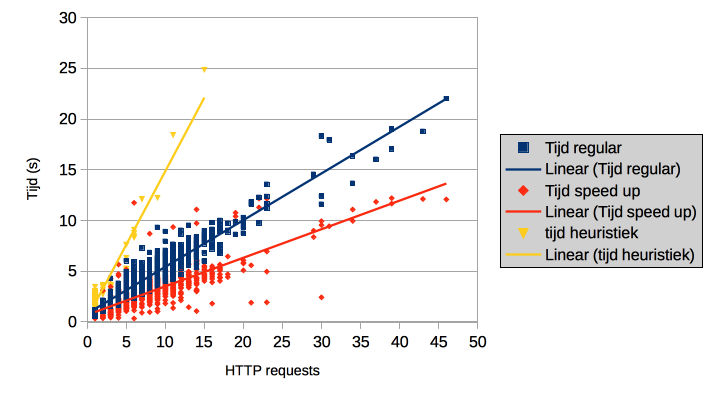
\includegraphics[width=0.5\textwidth]{tijdmetcachingvolgensaantalrequests}\label{fig:tijdmetcachingvolgensaantalrequests}}
  %\caption{Bovenstaande grafieken bevestigen de hypothese dat hoe meer connecties nodig zijn, hoe meer bandbreedte vereist wordt. Bijgevolg is er meer tijd nodig om een route te berekenen.}
\end{figure}
Bovenstaande grafiek (\ref{fig:aantalrequestsvolgensconnecties} toont aan dat het aantal requests lineair afhankelijk is met het aantal connecties. Ook grafiek \ref{fig:tijdmetcachingvolgensaantalrequests}) toont een lineair verband tussen de tijd en het aantal requests. Enkel requests met connecties zijn in rekening gebracht. Voordat connecties effectief opgevraagd worden, stuurt de cli\"ent een request om de juiste context op te vragen. Door de kleine grootte (1495 kB) en het feit dat dit bij alle technieken wordt gedaan, worden deze requests verwaarloosd. Beide figuren (\ref{fig:aantalrequestsvolgensconnecties} en \ref{fig:tijdmetcachingvolgensaantalrequests}) bevestigen de hypothese dat hoe meer connecties nodig zijn, hoe meer bandbreedte vereist wordt. Bijgevolg is er meer tijd nodig om een route te berekenen. In volgende subsectie wordt de snelheid getest in functie van de afstand.

\subsection{Snelheid}
Om de snelheid te meten van de verschillende technieken werden er 900 random routes gegenereerd. Volgende paragrafen tonen aan of er een groot verschil in performantie is afhankelijk van client-side caching.

\subsubsection{Met caching}
 
\begin{figure}[h!]
\centering
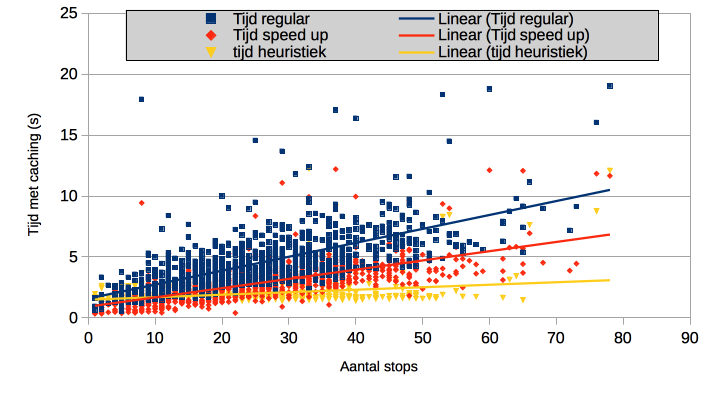
\includegraphics[width=0.5\textwidth]{tijdmetcachingvolgensaantalstops}
\caption{De tijd om een route te berekenen in functie van het aantal stops voor de NMBS.}
\label{tijdmetcachingvolgensaantalstops}
\end{figure}

Op grafiek \ref{tijdmetcachingvolgensaantalstops} is te zien hoe sterk de verschillende technieken schalen in snelheid ten opzichte van het aantal stops. 
De snelste techniek is die met de heuristiek. Daarna volgt de speed-up techniek en oorspronkelijke techniek met basic LCF's. Bij de heuristische techniek zijn de queries waarvoor geen optimale route gevonden werden, weggelaten. Dit zijn queries waarvoor meer dan 20 requests gestuurd zijn zonder enig resultaat. Meestal zijn dit ook moeilijkere queries, bijvoorbeeld buitenlandse stations zijn moeilijker bereikbaar. Deze moeilijkere queries brengen de grootste tijd met zich mee dus de werkelijke snelheid ligt gemiddeld wat hoger. 78 \% van de queries zijn gelukt met de heuristische methode.
De huidige implementatie die enkel basic LCF's gebruikt is overduidelijk de traagste. De speed-up techniek is zoals verwacht iets sneller. Bij uitschieters is er een groot verschil van enkele seconden tijd te merken tussen basic LCF's en de speed-up techniek. In tabel \ref{table:gemiddeldesnelheid} staat een overzicht van de gemiddelde snelheid per query. Zoals je kan zien kan de speed-up en heuristische methode ongeveer dubbel zoveel queries oplossen in dezelfde tijd als de basis methode met basic LCF's.
\begin{table}[htbp]
\centering
\begin{tabular}{ | c || c | c | c | }
 &  Basis methode & Speed-up & Heuristiek \\ \hline
  Gemiddelde snelheid (s/query) & 4.54 & 2.87 & 1.96 \\
\hline
\end{tabular}
\caption{Percentage nuttige connecties ten op zichte van alle gescande connecties voor elke techniek.}
\label{table:gemiddeldesnelheid}
\end{table}

De snelheid van de heuristiek is een stuk groter en constanter dan de andere twee technieken. Om dit te kunnen benaderen met de speed-up techniek, hebben we de paginagrootte voor de volgende test vergroot van 30 naar 40 minuten. De fragmentgrootte blijft weliswaar even groot.

Figuur \ref{tijdmetcachingvolgensafstand} toont aan dat het aantal stops overeenkomt met de afstand tussen begin- en eindpunt.

\begin{figure}[h!]
\centering
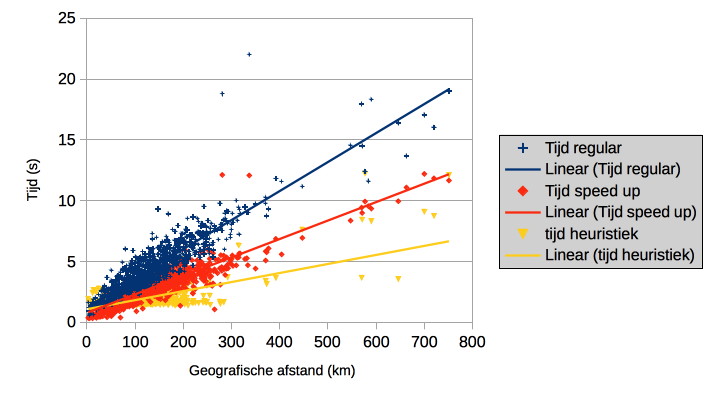
\includegraphics[width=0.5\textwidth]{tijdmetcachingvolgensafstand}
\caption{Verband tussen afstand begin-en eindpunt en tijd om te berekenen}
\label{tijdmetcachingvolgensafstand}
\end{figure}

\subsubsection{Zonder caching} 

\begin{figure}[h!]
\centering
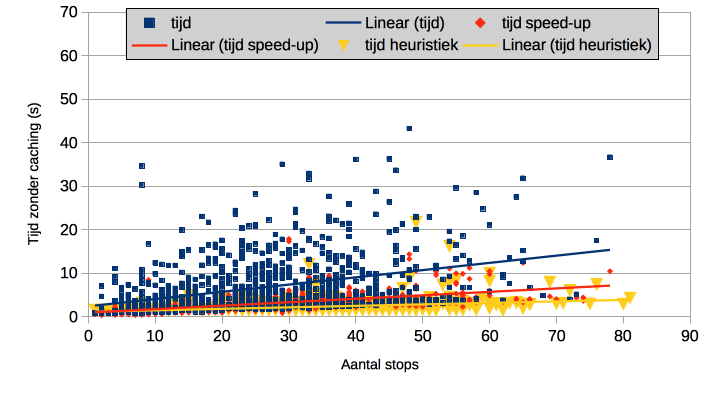
\includegraphics[width=0.5\textwidth]{tijdzondercachingvolgensaantalstops}
\caption{tijdzondercachingvolgensaantalstops}
\label{tijd zonder caching volgens aantal stops}
\end{figure}

Figuur \ref{tijdzondercachingvolgensaantalstops} toont de snelheid zonder client-side caching aan. In vergelijking met de vorige grafiek (\ref{tijdmetcachingvolgensaantalstops}) is er een groter verschil tussen basic LCF's en de speed-up techniek. Dit is te wijten aan de grotere fragmentgrootte in vergelijking met vorige test. In figuur \ref{routeduurinfunctievantijd} zie je dat de meeste routes tussen de 0 en 200 minuten liggen. Een grotere fragmentgrootte zorgt ervoor dat in minder requests het resultaat bekomen kan worden.

\begin{figure}[h!]
\centering
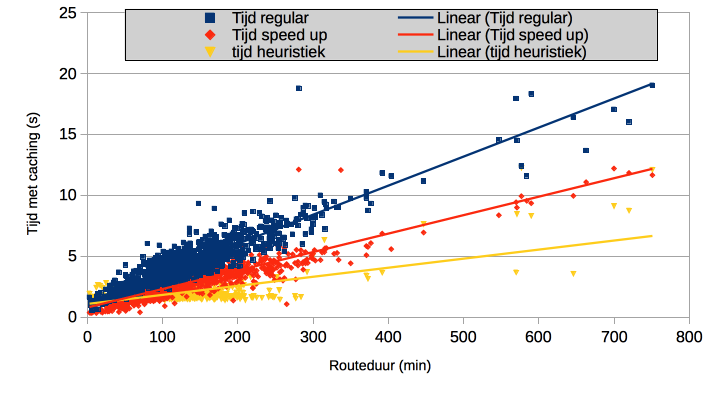
\includegraphics[width=0.5\textwidth]{routeduurinfunctievantijd}
\caption{De tijd om routes te berekenen in functie van de routeduur.}
\label{routeduurinfunctievantijd}
\end{figure}

De snelheid bij client-side routeplanning hangt niet alleen af van het aantal connecties, maar ook het aantal requests. Door een grotere fragmentgrootte te kiezen, moeten er minder requests gestuurd worden en kan het resultaat sneller berekend worden.

\subsection{Effici\"entie}
CSA gebruikt maar een beperkt aantal van de gescande connecties om een minimale overspannende boom te berekenen. De gegevens uit \ref{table:efficientie} tonen aan dat de speed-up techniek de effici\"entie van het aantal nuttige connecties verdubbelt in vergelijking met de originele implementatie. Merk hier ook op dat de heuristiek enkel rekening houdt met 80\% van de queries, die relatief makkelijker op te lossen waren, en dus een hogere score bekomt dan de speed-up techniek. 

\begin{table}[htbp]
\centering
\begin{tabular}{ | c || c | c | c | }
 &  Basis methode & Speed-up & Heuristiek \\ \hline
  Nuttige connecties (\%) & 0.026 & 0.047 & 0.064 \\
\hline
\end{tabular}
\caption{Percentage nuttige connecties ten op zichte van alle gescande connecties voor elke techniek.}
\label{table:efficientie}
\end{table}

\subsection{Dataverbruik}
\label{dataverbruik-heuristiek}

Naast effici\"entie is ook dataverbruik een belangrijk aspect bij routeplanning. Figuur \ref{table:dataverbruikheuristischemethode} geeft een overzicht hoeveel data er gemiddeld verbruikt wordt met hun onderlinge percentages. 

\begin{table}[htbp]
\centering
\begin{tabular}{ | c || c | c | c | }
 & Basis methode & Speed-up & Heuristiek \\ \hline
  Dataverbruik (MB) & 2.69 & 1.68 & 1.97 \\
  Percentage & 1 & 0.62  & 0.73 \\
\hline  
\end{tabular}
\caption{Percentage dataverbruik voor elke techniek.}
\label{table:dataverbruik}
\end{table}

\subsection{Serverbelasting}

In deze laatste test onderzoeken we de tijd die de server nodig heeft om connecties op te halen uit een databank. Hiervoor hebben we voor elke $K$, het maximaal aantal overstappen, en verschillende tijdsintervallen de gemiddelde tijd berekend om connecties op te halen. Zoals je kan zien in \ref{straalafstand} heeft de server minder last als er meer connecties moeten teruggegeven worden. Hoe groter de straal en hoe groter het tijdsinterval, hoe sneller antwoord kan teruggegeven worden.

\begin{figure}[h!]
\centering
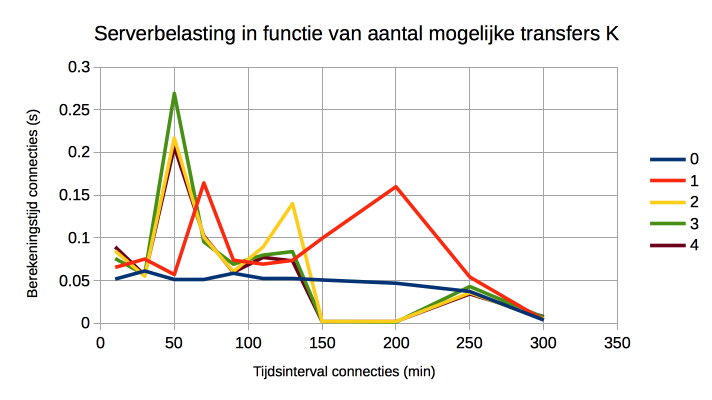
\includegraphics[width=0.8\textwidth]{straal-afstandgraf}
\caption{}
\label{straalafstand}
\end{figure}

\section{Conclusie}

\begin{table}[htbp]
\centering
\begin{tabular}{ | c || c | c | c | }
 Methode & Snelheid (query/s) & Dataverbruik (MB) & Optimaal  \\ \hline
  Basis & 15.74 & 2.69 & ja \\
  Speed-up & 28.70 & 1.68 & ja \\
  Heuristiek & 32.89 & 1.97 & nee \\
\hline  
\end{tabular}
\caption{Overzicht van de verschillende metrieken per techniek.}
\label{table:dataverbruik}
\end{table}



